\maketitle
\tableofcontents
\newpage

\section{Zielsetzung}
Ziel dieses Versuches ist es, gedämpfte und erzwungene Schwingungen zu untersuchen.
\section{Theorie}
Ein Schwingkreis besteht in seiner einfachsten Form aus einem Kondensator mit der Kapzität
$C$ und einer Spule mit der Induktivität $L$. Die Energie in diesem Schwingkreis oszilliert
zwischen den beiden Energiespeichern und hat als mögliche Maxima ein maximales magnetisches
Feld in der Spule und einen maximal aufgeladenen Kondensator. Falls ein idealer Draht
vorliegt, wird diese $\textbf{ungedämpfte Schwingung}$ für $t \to \infty$ unverändert schwingen.
\subsection{Gedämpfte Schwingung}
\label{sec:gedaempfteSchwingung}
\begin{figure}
  \centering
  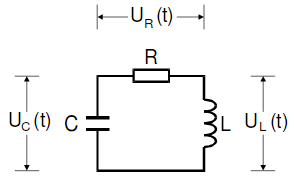
\includegraphics[scale=0.6]{gSchwingkreis.png}
  \caption{Schaltbild eines gedämpften Schwingkreises \cite{anleitung}.}
  \label{fig:1}
\end{figure}

Falls nun aber ein endlicher Widerstand $R$ in den Schaltkreis eingebaut wird, siehe \ref{fig:1},
dann wird ein Teil der elektrischen Energie an diesem ohmschen Widerstand in Wärme umgewandelt.
Damit fallen die Amplituden der Spannung und des Stromes mit der Zeit ab und es entwickelt sich
eine $\textbf{gedämpften Schwingung}$. Das Gesetz zwischen der Absinken der Amplitude und der Zeit
lässt sich aus dem zweiten Kirchhoffschen Gesetz, mit den Spannungen aus Abbildung \ref{fig:1},
herleiten
\begin{equation}
    U_R (t) + U_L (t) + U_C (t) = 0 \, .
    \label{eqn:1}
\end{equation}
Daraus entwickelt man eine lineare homogene Differentialgleichung 2. Ordnung der Form
\begin{equation}
    \ddot{I}(t) + \frac{R}{L} \ddot{I}(t) +
    \frac{1}{LC} \, I(t) = 0 \, ,
    \label{eqn:2}
\end{equation}
welche als Lösung
\begin{equation}
  I'(t) = e^{-2 \pi \mu t} \left(A e^{i 2 \pi \nu t} + B e^{-i 2 \pi \nu t}\right)
  \label{eqn:3}
\end{equation}
mit $A$ und $B$ als beliebige Zahlen aus $\mathbb{C}$ und den Abkürzungen
\begin{equation*}
    \begin{split}
        2 \pi \mu = \frac{R}{2L} \\
        2 \pi \nu = \sqrt{\frac{1}{LC} - \frac{R^2}{4L^2}}
    \end{split}
\end{equation*}
besitzt. Für den weiteren Verlauf ist es erforderlich zu ermitteln, ob $\nu$
reell oder imaginär ist. Deshalb wird eine Fallunterscheidung ausgeführt:
\begin{itemize}
  \item $\nu$ ist reell:

    Damit in diesem Fall $I'(t)$ reell wird, muss $A = \overline{B}$ gelten. Mit
    geeigneten Ansätzen erhält man schließlich
    \begin{equation}
        I(t) = A_0 \, e^{-2 \pi \mu t} \, \symup{cos} \left(2 \pi f t + \eta \right)
        \label{eqn:4}
    \end{equation}
    mit $A_0$ und $\eta$ als beliebige Zahlen aus $\mathbb{R}$ und $f$ als Frequenz der
    Schwingung. Gleichung \eqref{eqn:4} stellt eine Schwingungsgleichung für eine
    $\textbf{gedämpfte Schwingung}$ dar, deren Amplitude offensichtlich exponentiell gegen 0 strebt.
    Für die Schwingungsdauer ergibt sich
    \begin{equation}
      T = \frac{1}{f} = \frac{2 \pi}{\sqrt{\frac{1}{LC} - \frac{R^2}{4L^2}}} \, .
      \label{eqn:5}
    \end{equation}
    Die Abnahmegeschwindigkeit steckt im Exponenten der e-Funktion in \eqref{eqn:4},
    nämlich im $\mu$. Daraus lässt sich die Abklingdauer $T_\symup{ex}$ definieren
    \begin{equation}
        T_\symup{ex} = \frac{1}{2 \pi \mu} = \frac{2L}{R} \, .
        \label{eqn:6}
    \end{equation}
  \item $\nu$ ist imaginär:

    Gleichung \eqref{eqn:3} besteht nur noch aus vollständig reellen Exponentialfunktionen,
    sodass \eqref{eqn:4} keinen oszillatorischen Anteil besitzt. Dies nennt man
    aperiodische Dämpfung. Abhängig von $A$ und $B$ strebt $I(t)$ monoton gegen 0 oder
    erreicht noch einen Extremwert. Für das Experiment von Bedeutung ist der Spezialfall
    \begin{equation}
        \frac{1}{LC} = \frac{R_{\symup{ap}}^2}{4L^2} \, ,
        \label{eqn:7}
    \end{equation}
    der $\textbf{aperiodischer Grenzfall}$ heißt und für den $f = 0$ ist. Die Amplitude des Stroms strebt maximal schnell
    gegen 0 und besitzt keinen Überschwinger.
\end{itemize}
\subsection{Erzwungene Schwingung}
\begin{figure}
  \centering
  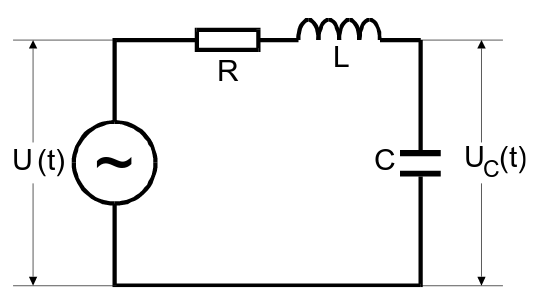
\includegraphics[scale=0.4]{eSchwingkreis.png}
  \caption{Schaltbild einer erzwungenen Schwingung \cite{alt}.}
  \label{fig:2}
\end{figure}
Nun wird der $RCL$-Schwingkreis aus Kapitel \ref{sec:gedaempfteSchwingung} um eine
Wechselstromquelle $U(t)$ erweitert, wie in Abbildung \ref{fig:2} zu sehen. Diese regt den Schwingkreis
mit einer eigenen Frequenz zusätzlich an. Nach einer gewissen Einschwingzeit wird der Schwingkreis
mit derselben Frequenz wie die Wechselstromquelle schwingen.
Mit
\begin{equation*}
    U(t) = U_0 \, e^{i \omega t}
\end{equation*}
wird die Differentialgleichung \eqref{eqn:2} verändert zu
\begin{equation}
    LC \ddot{U}_C + RC \ddot{U}_C + U_C = U_0 \, e^{i \omega t} \, .
    \label{eqn:8}
\end{equation}
Um zu ermitteln, wie die Amplitude $U_{C0}$ der Kondensatorspannung mit dem Phasenunterschied
von der Erregerspannung mit der Amplitude $U_0$ und ihrer Frequenz abhängen, nimmt man den Ansatz
\begin{equation*}
  U_C(\omega, t) = U_{C0}(\omega) \, e^{i \omega t}
\end{equation*}
und setzt ihn in \eqref{eqn:8} ein. Damit erhält man für die Amplitude
\begin{equation}
    U_{C0} = \frac{U_0 \left(1 -LC \omega^2 - i \omega RC \right)}{\left(1 - LC \omega^2 \right)^2 + \omega^2 R^2 C^2}
    \label{eqn:9}
\end{equation}
und für die Phasenverschiebung $\phi (\omega)$ zwischen $U_C(t)$ und $U(t)$
\begin{equation}
    \phi (\omega) = \symup{arctan} \left(\frac{-\omega R C}{1 - LC \omega^2}\right) \, .
    \label{eqn:10}
\end{equation}
Für die Frequenzen $\omega_1$ und $\omega_2$ bei denen die Phasenverschiebung genau
$\frac{\pi}{4}$ bzw. $\frac{3\pi}{4}$ beträgt, gilt dann nach \eqref{eqn:10}
\begin{equation}
  \omega_{1,2} = \pm \frac{R}{2L} + \sqrt{\frac{R^2}{4L^2} + \frac{1}{LC}}
  \label{eqn:15}
\end{equation}
Mit \eqref{eqn:9} erhält man für die Kondensatorspannung in Abgängigkeit von $\omega$ die sogennante
Resonanzkurve
\begin{equation}
  U_C(\omega) = \frac{U_0}{\sqrt{\left(1- LC \omega^2\right)^2 + \omega^2 R^2 C^2}} \, .
  \label{eqn:11}
\end{equation}
An Gleichung \eqref{eqn:11} lässt sich erkennen, dass die Kondensatorspannung für
$\omega \to \infty$ gegen 0 und für $\omega \to 0$ gegen $U_0$ geht. Allerdings
gibt es eine Frequenz, für die die Kondensatorspannung maximiert wird, sodass $U_C > U_0$ gilt. Dies wird als
Resonanz mit der Resonanzfrequenz
\begin{equation}
  \omega_\symup{res} = \sqrt{\frac{1}{LC} - \frac{R^2}{2L^2}}
  \label{eqn:12}
\end{equation}
bezeichnet. Falls nun die Resonanzfrequenz ungefähr der Frequenz des ungedämpften Schwingkreises
$\omega_0 = \frac{1}{LC}$, d.h. dass in \eqref{eqn:12} $\frac{1}{LC} >> \frac{R^2}{2L^2}$ gilt,
entspricht, so nennt man dies schwache Dämpfung. Für diesen Fall wird $U_C$ um den Faktor
\begin{equation}
  q = \frac{1}{\omega_0 RC}
  \label{eqn:13}
\end{equation}
größer als $U_0$. \eqref{eqn:13} nennt man auch die $\textbf{Güte q}$ des Schwingkreises.

Eine weitere wichtige Größe ist die Breite der Resonanzkurve aus Formel \eqref{eqn:11}.
Sie wird aus der Differenz der beiden Frequenzen $\omega_+$ und $\omega_-$ gewonnen,
welche sich dadurch auszeichnen, dass $U_C(\omega_+)$ und $U_C(\omega_-)$ um den Faktor
$\frac{1}{\sqrt{2}}$ kleiner sind als das Maximum aus \eqref{eqn:13}. Mit der Näherung
\begin{equation*}
  \frac{R^2}{L^2} << \omega_0^2
\end{equation*}
folgt für die Differenz der Frequenzen
\begin{equation}
    \omega_+ - \omega_- \approx \frac{R}{L} \, .
    \label{eqn:14}
\end{equation}

\section{Durchführung}

\subsection{Versuchsaufbau}

\subsection{Versuchsdurchführung}
\section{Auswertung}

\section{Diskussion}
\newpage
\nocite{*}
\printbibliography
